	\documentclass[12pt,a4paper]{article}
	\usepackage[utf8]{inputenc}
	\usepackage[portuguese]{babel}
	\usepackage[T1]{fontenc}
	\usepackage{amsmath}
	\usepackage{amsfonts}
	\usepackage{amssymb}
	\usepackage{graphicx}
	\usepackage[left=2.5cm,right=2.5cm,top=2.5cm,bottom=2.5cm]{geometry}
	\author{Paulo Batista da Costa}
	\title{Laudo PBR refente ao projeto II }
	
	\begin{document}
	
        \begin{titlepage}
        \LARGE
        	\begin{center}
        	\vspace{5cm} 
        	\textbf{Universidade Tecnológica Federal do Paraná \\ \vspace{1.8cm}}
        	
\includegraphics[scale=0.35]{logoutfpr.jpg} \\ \vspace{1.8cm}
        	\textit{Engenharia de Software II} \vspace{2cm} \\
        	Paulo Batista da Costa \\ 1509764 \vspace{2cm} \\ 
        	PROJETO 2 - PLANEJAMENTO DE DESENVOLVIMENTO DE SOFTWARE \vspace{2cm} \\
        	Departamento de Ciência da Computação (DACOM) 
        	
        	\end{center}
        \end{titlepage}	
	
		\tableofcontents
		
		
		\newpage
		\section{Da Natureza Deste Documento}
		\paragraph{} Este documento é referente ao planejamento de atividades de desenvolvimento de software do projeto 2. Tal projeto é proposto como base de atividades na disciplina de engenharia de software II. Desse modo, o objetivo deste documento é explicitar o conjunto de atividades de desenvolvimento do projeto 2 de forma a dividi-lo em conjunto de tarefas ou grupo de atividades que serão executadas. 
		
		\paragraph{} Por sua vez, o grupo de desenvolvimento seguirá este plano como base fundamental para caminhar o desenvolvimento. Aqui também é analisado uma estimativa de tempo para cada parte do processo de elaboração de atividades (compatível com a estimativa de tempo realizada previamente). Apenas a critério de informação, o desenvolvimento das atividades darão início  a partir do momento em que este documento estiver lançado no repositório de desenvolvimento.
		\section{Descrição de Atividades}
		\paragraph{} A primeira etapa do planejamento de software é a divisão do desenvolvimento em etapas. Assim, o conjunto tem partes distinguíveis entre si e estas são distribuídas de maneira sensata aos colaboradores do projeto. Cada etapa de desenvolvimento será de responsabilidade de um integrante do projeto. Na subseção a seguir estão explícitas as etapas e as respectivas distribuições de tarefas.
		\subsection{Etapa 1: Diagramação}
		\paragraph{}Nesta etapa está explícito o planejamento do desenvolvimento de atividades relacionadas a elaboração de documentos para a implementação, ou seja, criação de diagramas que auxiliem e ditem as regras de negócio, estas obtidas através do processo de abstração informacional a partir da documentação referente ao projeto 2.
		\paragraph{} Esta etapa é destinada ao projetista do sistema. Ele terá cerca de 23.16 horas para a elaboração total  de todos os documentos. 
		\subsubsection{Diagramação: Casos de Uso -- A}
		\paragraph{}Esta etapa compreende a elaboração do diagrama de caso de uso, este consiste  na focalização das funcionalidades que o projeto abrangerá. Nesta fase de diagramação o projetista deverá consumir em torno de 3,16 horas, isto de acordo com a realização da estimativa de tempo previamente realizada.
		\subsubsection{Diagramação: Diagramas de Classe -- B}
		\paragraph{}Esta etapa compreende a elaboração do diagrama de classe. Esta etapa é mais profunda que a anterior, pois determina as entidades inerentes ao sistema. Além disso, determina como o sistema está interconectado e dá noção de complexidade de implementação ao grupo de desenvolvimento. Aqui a estimativa de tempo é de 4,5 horas consumidas pelo projetista do sistema.
		\subsection{Sequenciamento de atividades: Ordem de atividades do projetista}
		\paragraph{} Deve ser explicitado que necessariamente o projetista elaborará primeiramente o diagrama de casos de uso previamente ao diagrama de classes. Isto, pois o primeiro dará a verdadeira faceta do projeto e suas reais funcionalidades. Enquanto o segundo depende do primeiro, pois para ser implementado componentes do projeto, é necessário que se saiba o que de fato é necessário que o sistema realize.
		\paragraph{} Portanto, a realização de atividades possui até aqui o seguinte sequenciamento: \\
		\begin{table}[!ht]	
		\centering
		\begin{tabular}{|c|c|c|}
		\hline 
		Atividade & Atividade precedente & Duração Estimada (Horas) \\ 
		\hline 
		A & - & 3,16 \\ 
		\hline 
		B & A & 4,5 \\ 
		\hline 
		\end{tabular}
		\caption{tabela de sequenciamento de atividades: Diagramação.} 
		\end{table}
		\paragraph{} Como pode ser visto na tabela, a quantidade de horas estimadas nessa etapa de desenvolvimento é de 7,56 horas. Por sua vez, seu sequenciamento segue a ordem de A para B, sendo A a diagramação dos casos de uso e B a realização dos diagramas de classe. \\
		\begin{figure}[!ht]
		\centering
		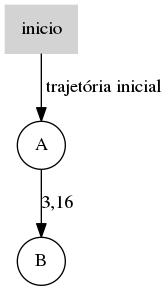
\includegraphics[scale=0.5]{001.png}
		\caption{Sequenciamento de A para B, os números são referentes às horas previstas}
		\end{figure}	
		\subsection{Etapa 2: Implementação}	
		\paragraph{} Aqui é descrito o sequenciamento de atividades a partir do momento em que se tem em mãos a diagramação completa dos requisitos funcionais a partir da documentação. Em outras palavras, nesta etapa o projetista já gerou documentos suficientes para que o programador interprete o que será implementado. A implementação será dividida em três etapas, sendo a primeira referente a implementação das classes que compõem o sistema e a segunda referente ao banco de dados que deverá suportar o armazenamento informacional. A última etapa é referente à interface gráfica e será tratada no final.O tempo total previsto para esta etapa é de 36,5 horas.         	
		\subsubsection{Implementação: Classes -- C}
		\paragraph{} Nesta etapa, de acordo com o que pode ser visto na previsão de consumo de tempo, o programador terá cerca de 15,5 horas para concluir a implementação de classes do sistema. Esta é necessariamente a primeira etapa do desenvolvimento do sistema, sendo que a modelagem e implementação do banco de dados será a etapa consecutiva a esta.
		\subsubsection{Implementação: Banco de Dados -- D}
		\paragraph{} Esta é a segunda etapa do desenvolvimento, sendo que para esta é previsto um consumo de tempo de aproximadamente 7,17 horas. 
		\subsubsection{Implementação: Interface Gráfica -- E}
		\paragraph{} Última etapa do desenvolvimento, na qual está previsto o gasto de 13,83 horas de implementação.
		\subsection{Sequenciamento de Atividades: Ordem de atividades do Programador}
		\paragraph{}O programador seguirá as etapas descritas anteriormente afim de manter a organização do processo de desenvolvimento parcial das partes do sistema. Estas serão distinguíveis entre si quando ao contexto de implementação, bem como, sua representatividade perante ao sistema como um todo. A tabela a seguir exibe o sequenciamento até então tido nas etapas de desenvolvimento.
        \begin{table}[!ht]
        \centering
        \begin{tabular}{|c|c|c|}
        \hline 
        Atividade & Atividade Prescedente & Duração Estimada (Horas) \\ 
        \hline 
		A & - & 3,16 \\ 
		\hline 
		B & A & 4,5 \\  
        \hline 
        C & A,B & 15,5 \\ 
        \hline 
        D & C & 7,17 \\ 
        \hline 
        E & C,D & 13,83 \\ 
        \hline 
        \end{tabular} 
        \end{table} 
        \begin{figure}[!ht]       		
			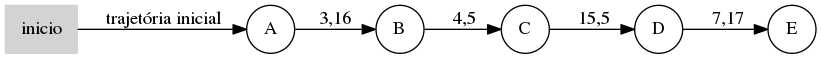
\includegraphics[scale=0.5]{002.png}
			\caption{Sequenciamento de Atividades: adicionadas as três etapas de implementação de código. Isto sendo C a implementação de Classes, D a implementação de Banco e E a de interface gráfica. Os números são as horas consumidas}
			\end{figure}
		\subsection{Etapa 3: Realização de testes -- F}
		
		
		\paragraph{} Esta etapa é responsabilidade do \textit{tester}. Ele deverá encontrar o maior número de erros possíveis. Esta etapa só será aplicada após o término das implementações massivas do sistema. Segundo a estimativa, é previsto que o responsável pela etapa consumirá cerca de 5,3 horas para desenvolver testes de performance, confiabilidade, integridades e dentre outros aspectos do sistema. Após este passo, o \textit{relatará ao gerente} os erros encontrados no sistema para que este seja ao programador para correções.
		\subsubsection{Sequenciamento: Ordem de Atividades até a etapa do \textit{tester}}
		Aqui verifica-se o sequenciamento do desenvolvimento até a etapa do \textit{tester}
		\begin{table}[!ht]
		\centering
        \begin{tabular}{|c|c|c|}
        \hline 
        Atividade & Atividade Prescedente & Duração Estimada (Horas) \\ 
		 \hline 
		A & - & 3,16 \\ 
		\hline 
		B & A & 4,5 \\         
        \hline 
       
        C & A,B & 15,5 \\ 
        \hline 
        D & C & 7,17 \\ 
        \hline 
        E & C,D & 13,83 \\ 
        \hline 	
        F & C,D,E &  5,3 \\
        \hline
        \end{tabular}	 
		\end{table}
		
		\begin{figure}[ht!]
			\centering
			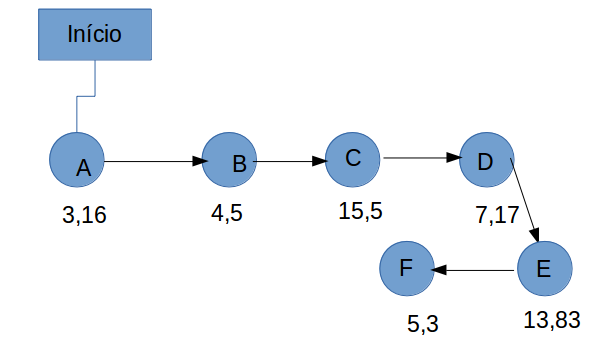
\includegraphics[scale=0.5]{003.png}
			\caption{Sequenciamento de atividades: os números atrelados aos nós são relativos ao consumo em horas por atividade}
		\end{figure}
		
		
		\subsection{Etapa 4: Correções de \textit{bugs} e outros defeitos -- G}
		\paragraph{} Esta etapa é referente à correção de defeitos encontrados pelo \textit{tester}. Assim, é um dever do programador realizar a manutenção. Por sua vez, este terá um tempo aproximadamente de 8,5 horas para conclusão.	Com isto, encerram-se as etapas de produção e o gerente fará uma avaliação final do produto (verificar se o produto tem qualidade mínima e atende os requisitos funcionais)
		\subsection{Sequenciamento: Da ordem de atividades até a etapa de correção pelo programador}
		Aqui verifica-se o desenvolvimento sequencial até a etapa de correção de \textit{bugs}.
		\begin{table}[!ht]
		\centering
        \begin{tabular}{|c|c|c|}
        \hline 
        Atividade & Atividade Precedente & Duração Estimada (Horas) \\ 
		 \hline 
		A & - & 3,16 \\ 
		\hline 
		B & A & 4,5 \\         
        \hline 
        C & A,B & 15,5 \\ 
        \hline 
        D & C & 7,17 \\ 
        \hline 
        E & C,D & 13,83 \\ 
        \hline 	
        F & C,D,E &  5,3 \\
        \hline
        G & F & 8.5 \\
        \hline
        
        \end{tabular}	
        \caption{Tabela de atividades que expressa todos os passos de desenvolvimento do projeto.}
		\end{table}
		\subsection{Etapa 5: Validação de Correções -- H}
		\paragraph{} Esta etapa compete ao gerente. Ele deverá assegurar que o sistema está pronto para o uso. A partir daqui está definido o término das atividades de desenvolvimento e o produto será liberado para o cliente. Devido a este fato, não convém uma estimativa de tempo ou assegurar espaço em cronograma, pois esta eventualidade é apenas um \textit{checkpoint} do término e da entrega ao cliente.
 		\section{Da Tabela de Atividades}
		\paragraph{} As tabelas de atividade expressam o sequenciamento de tarefas ao longo do projeto. Entretanto, além delas é disponibilizado a estrutura de um grafo que exibe desde o marco de início até o marco de entrega do produto (contendo as etapas intermediárias). Na seção a seguir, uma especificação maior do que foi elaborado neste planejamento de desenvolvimento de software.
		
		
		A seguir, a tabela de atividades (porém com um detalhamento maior): 
		
		
		\begin{table}[!ht]
				\centering
				\begin{tabular}{|c|c|c|c|}
					\hline 
					Atividade & Descrição& Atividade Precedente & Duração Estimada (Horas) \\ 
					\hline 
					A & D. Casos de Uso & - & 3,16 \\ 
					\hline 
					B & D. de Classes& A & 4,5 \\         
					\hline 
					C & I. Classes& A,B & 15,5 \\ 
					\hline 
					D & I. BD& C & 7,17 \\ 
					\hline 
					E & I. interface & C,D & 13,83 \\ 
					\hline 	
					F & Testes & C,D,E &  5,3 \\
					\hline
					G & C. de Defeitos & F & 8.5 \\
					\hline 
					H & Validação de Software & G & -- \\ \hline 
					
				\end{tabular}	
				\caption{quadro detalhado do sequenciamento de atividades}
		\end{table}
		\paragraph{} Percebe-se que o tempo total estimado em horas para a execução do projeto é de 57,96 horas. Isto é apenas uma estimativa da quantia total. A seguir o grafo sequencial de tarefas e posteriormente a elaboração do cronograma de desenvolvimento incluindo datas estipuladas para conclusões de etapas de desenvolvimento (Do início ao término -- todas as etapas)
		
		\section{Grafo determinístico: Sequenciamento estratégico de atividades}
		\paragraph{} Aqui está explicitado a versão completa da estrutura que define a sequência de atividades do projeto. Tal não foi definida com o critério do custo de menor tempo (utilização do conceito de caminho crítico), mas sim com base no aspecto de desenvolvimento incremental e do uso de \textbf{MVC} -- \textit{Model,View,Controller}. Assim, o critério de construção da sequencia de atividades pode ser entendido como um grafo que define um caminho de dependências do projeto (leva-se em consideração que se tem disponível apenas um programador)
		
		A seguir, o grafo explicitado (os pesos estão rotulados em seus nós, e não em arestas -- meramente ilustrado para compreensão da sequencia de etapas): 
		
		\begin{figure}[!ht]
			\centering
			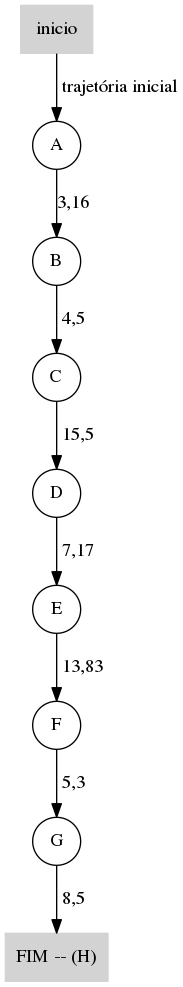
\includegraphics[scale=0.5]{004.png}
		\end{figure}
		
		\section{Cronograma de atividades}
		\paragraph{} No cronograma de atividades não será especificado qual horário ou dia o participante do projeto deverá desenvolver. Entretanto, como é necessário ter um controle do processo de desenvolvimento para que este siga prazos e venha a fazer parte de um rol de metas é necessário estipular prazos. A única obrigação referente a datas é a entrega do trabalho no tempo correto e juntamente entregar as marcações de dias e horas trabalhadas. Isto para verificação a respeito das estimativas e da eficiência do planejamento realizado.
		
		Segue o cronograma: 
		
		\begin{enumerate}
			\item Desenvolvimento de Casos de Uso: Entrega em 17/06/16
			\item Desenvolvimento de Diagrama de Classe: Entrega em 17/06/16
			\item Implementação de Classes: Entrega em 24/06/16
			\item Implementação de Banco de Dados:Entrega em 26/06/16
			\item Implementação de Interface Gráfica: 30/06/16
			\item Realização de testes: Entrega 02/07/16
			\item Correção de defeitos: Entrega 05/07/16
			\item Avaliação do produto e entrega: 06/07/16  
		\end{enumerate}
		
		\subsection{Justificativas do Cronograma de atividades}
		\paragraph{} Como o processo de desenvolvimento é simplificado quanto as atividades concomitantes, pelo fato de que as atividades possuem dependência entre si e a forma de desenvolvimento é similar às metodologias tradicionais, só há um caminho na rede. Assim, não foi necessário utilizar métodos complexos para calcular qual o melhor caminho a ser tomado na decisão da sequencia de atividades.
		\paragraph{}Isto define que este caminho único seja o caminho crítico. A respeito das datas, é tido como ponto de partida o dia de hoje (15/06/16), dia em que este documento foi lançado. Assim, a primeira etapa corrente será o desenvolvimento de diagrama de casos de uso. A respeito da quantidade de dias, foi tomado a decisão de dar um tempo extra, considerando possíveis fatores humanos que os desenvolvedores possuem rotinas fora do projeto.  Assim, o planejamento tem um cronograma que totaliza 22 dias. 
		\section{Plano de Contenção: Possíveis problemas do desenvolvimento}
		\paragraph{} Aqui considera-se que fatores humanos podem intervir no plano de desenvolvimento e possivelmente vir a decorrer na falha da execução das previsões de consumo de tempo, bem como, nas entregas nas datas previstas. Desse modo, cabe ao gerente estar ciente da situação dos membros da equipe e assumir a responsabilidade por elementos não concluídos ou falhos ao término do projeto. 
		\paragraph{} Por causa disso, é necessário salientar que o gerente intervirá em etapas do processo de desenvolvimento quando este analisar a deficiência na execução do plano de projeto.
		\section{Metodologia empregada: Como foi realizado este planejamento de desenvolvimento de software}
		\paragraph{}Este planejamento de software foi realizado com base em dois fatores de escolha organizacional: metodologia de desenvolvimento tradicional  e padrão arquitetural de software adotado. Tudo será elaborado de forma incremental e modular, sendo que uma etapa anterior sempre será subsídio da próxima etapa (principalmente quanto a implementação) e estas definem as atividades de software.
		\end{document}